%\documentclass[mathserif]{beamer}
\documentclass[handout]{beamer}
%\usetheme{Goettingen}
\usetheme{Warsaw}
%\usetheme{Singapore}
%\usetheme{Frankfurt}
%\usetheme{Copenhagen}
%\usetheme{Szeged}
%\usetheme{Montpellier}
%\usetheme{CambridgeUS}
%\usecolortheme{}
%\setbeamercovered{transparent}
\usepackage[english, activeacute]{babel}
\usepackage[utf8]{inputenc}
\usepackage{amsmath, amssymb}
\usepackage{mathtools}
\usepackage{dsfont}
\usepackage{graphics}
\usepackage{cases}
\usepackage{graphicx}
\usepackage{pgf}
\usepackage{epsfig}
\usepackage{amssymb}
\usepackage{multirow}	
\usepackage{amstext}
\usepackage[ruled,vlined,lined]{algorithm2e}
\usepackage{amsmath}
\usepackage{epic}
\usepackage{epsfig}
\usepackage{fontenc}
\usepackage{framed,color}
\usepackage{palatino, url, multicol}
\usepackage{listings}
%\algsetup{indent=2em}


\vspace{-0.5cm}
\title{Reinforcement Learning and Control}
\vspace{-0.5cm}
\author[Felipe Bravo Márquez]{\footnotesize
%\author{\footnotesize  
 \textcolor[rgb]{0.00,0.00,1.00}{Felipe José Bravo Márquez}} 
\date{ \today }




\begin{document}
\begin{frame}
\titlepage


\end{frame}


%%%%%%%%%%%%%%%%%%%%%%%%%%%


\begin{frame}{Introduction}
\scriptsize{
\begin{itemize}
\item In supervised learning, algorithms try to make their outputs mimic the labels $y$ given in the training set \footnote{These slides are based on \cite{ng2000cs229}.}. 
\item The labels give an unambiguous ``right answer'' for each of the inputs $x$.
\item In contrast, for many sequential decision making and control problems, it is very difficult to provide this type of explicit supervision to a learning algorithm.
\item For example, if we have just built a four-legged robot and are trying to program it to walk.
\item Initially we have no idea what the ``correct'' actions to take are to make it walk
\item Hence, we don't know how to provide explicit supervision for a learning algorithm to try to mimic.
\end{itemize}


} 

\end{frame}


\begin{frame}{Introduction}
\scriptsize{
\begin{itemize}
\item In the reinforcement learning framework, we povide our algorithms only a reward function.
\item This function indicates to the learning agent when it is doing well, and when it is doing poorly. 
\item In the four-legged walking example, the reward function might give the robot positive rewards for moving forwards, and negative rewards for either moving backwards or falling over.
\item It will then be the learning algorithm's job to figure out how to choose actions
over time so as to obtain large rewards.
\end{itemize}


} 

\end{frame}


\begin{frame}{Introduction}
\scriptsize{
\begin{itemize}
\item Reinforcement learning has been successful in applications as diverse as:
\begin{enumerate}
\scriptsize{
 \item autonomous helicopter flight
 \item robot legged locomotion
 \item cell-phone network routing
 \item marketing strategy selection
 \item factory control
 \item efficient web-page indexing}
 \end{enumerate}


\item Our study of reinforcement learning will begin with a definition of
the Markov decision processes (MDPs).
\item MDPs provide the formalism in which RL problems are usually posed.
\end{itemize}


} 

\end{frame}


\begin{frame}{Markov Decision Process (MDP)}
\scriptsize{
\begin{itemize}
\item A Markov Decision Process is a tuple: 
\begin{displaymath}
 (S,A,\{P_{SA}\},\gamma,R)
\end{displaymath}
where
\item $S$ is a set os states. (For example, in autonomous helicopter flight, $S$
might be the set of all possible positions and orientations of the helicopter.)
\item $A$ is a set of actions. (For example, the set of all possible directions in
which you can push the helicopter's control sticks.)

\end{itemize}


} 

\end{frame}


\begin{frame}{Markov Decision Process (MDP)}
\scriptsize{
\begin{itemize}
\item $P_{sa}$ are the state transition probabilites. For each state $s \in S$ and
action $a \in A$, $P_{sa}$ is a distribution over the state space, i.e., it gives the distribution over what states we will transition to if we take action $a$ in state $s$.

\begin{displaymath}
 \sum_{s'}P_{sa}(s')=1, \quad P_{sa}(s')\geq 0
\end{displaymath}

\item $\gamma \in [0,1)$ is a discount factor.

\item $R: S \rightarrow \mathcal{R}$  is a reward function.

\end{itemize}


} 

\end{frame}




\begin{frame}{Markov Decision Process (MDP)}
\scriptsize{
The dynamics of an MDP proceeds as follows:
\begin{itemize}
\item  We start in some state $s0$, and get to choose some action $a0 \in A$ to take in the MDP.
\item As a result of our choice, the state of the MDP randomly transitions to some successor state $s1$ , drawn according to $s1 \sim P_{s0a0}$.
\item Then, we get to pick another action $a1$.
\item As a result of this action, the state transitions again, now to some $s2 \sim P_{s1a1}$.
\item We then pick $a2$ , and so on. . . . 
\end{itemize}

Pictorially, we can represent this process as follows:


\begin{displaymath}
 so \xrightarrow{a0} s1 \xrightarrow{a1} s2 \xrightarrow{a2}  s3 \xrightarrow{a3} ..
\end{displaymath}



} 

\end{frame}


\begin{frame}{Example}
\scriptsize{
\begin{itemize}
\item Suppose that an agent is situated in the $4\times 3$ environment as shown in the Figure below: 


  \begin{figure}[h]
        	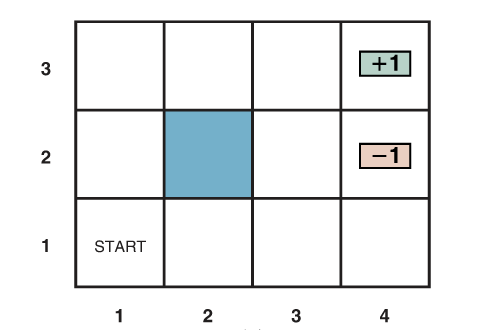
\includegraphics[scale = 0.4]{pics/example.png}
        \end{figure}

\item Beginning in the start state, it must choose an action at each time step. 

\item There 11 states ($S$) and four actions $A=\{N,S,E,W\}$.

\item The interaction with the environment terminates when the agent reaches one of the goal states, marked +1 or –1.

\end{itemize}


} 

\end{frame}


\begin{frame}{Example}
\scriptsize{
\begin{itemize}
\item The ``intended'' outcome occurs with probability 0.8, but with probability 0.2 the agent moves at right angles to the intended direction:

  \begin{figure}[h]
        	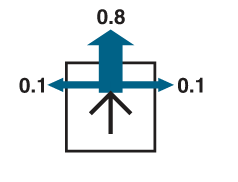
\includegraphics[scale = 0.4]{pics/example1.png}
        \end{figure}

\item For example:

 $P_{(3,1)N}((3,2))=0.8$ \\
 $P_{(3,1)N}((4,1))=0.1$ \\
 $P_{(3,1)N}((2,1))=0.1$ \\
 $P_{(3,1)N}((3,3))=0$ \\
... etc


\end{itemize}


} 

\end{frame}

\begin{frame}{Total Payoff}
\scriptsize{
\begin{itemize}
\item Upon visiting the sequence of states $s0 , s1 , ...$ with actions $a0, a1, ...,$ our
\textbf{total payoff} is given by:
\begin{displaymath}
 R(so)+\gamma R(s1)+\gamma^2R(s2)+...
\end{displaymath}
$0 \leq \gamma < 1$

\item Our goal in reinforcement learning is to choose actions over time so as to
maximize the expected value of the total payoff:

\begin{displaymath}
 E[R(so)+\gamma R(s1)+\gamma^2R(s2)+...]
\end{displaymath}

\item Note that the reward at timestep $t$ is discounted by a factor of $\gamma^t$.
\item Thus, to make this expectation large, we would like to accrue positive rewards as soon
as possible (and postpone negative rewards as long as possible). 
\item In economic applications where $R(\cdot)$ is the amount of money made, $\gamma$ also has a natural interpretation in terms of the interest rate (where a dollar today is worth
more than a dollar tomorrow).


\end{itemize}


} 

\end{frame}


\begin{frame}{Example}
\scriptsize{
\begin{itemize}
\item A collision with a wall results in no movement.

\item Transitions into the two terminal states have reward +1 and –1, respectively. \\
$R((4,3)) = +1$ \\
$R((4,2)) = -1$ \\
$R(S) = -0.02$ for all other states.

\item All other transitions have a reward of –0.02 (to avoid the robot wasting time).

\end{itemize}


} 

\end{frame}

%%%%%%%%%%%%%%%%%%%%%%%%%%%
\begin{frame}[allowframebreaks]\scriptsize
\frametitle{References}
\bibliography{bio}
\bibliographystyle{apalike}
%\bibliographystyle{flexbib}
\end{frame}  









%%%%%%%%%%%%%%%%%%%%%%%%%%%

\end{document}
